
\documentclass{article}
\usepackage{color}
\usepackage{amsmath}
\usepackage{subcaption}
\captionsetup{compatibility=false}
\usepackage{graphicx}
\usepackage{grffile}
\usepackage{epstopdf}
\begin{document}



\section{Model predictive control unconstrained}

\subsection{UAV dynamics}
For understanding the UAV's controller, it is important to understand the physical properties of UAV. It has 4 rotors, 


\subsection{MPC Introduction}
MPC is an advanced regulator. It using prediction of future states of the system to determine system input actions. This prediction runs constantly in a loop. Because of it's computational demands, it is used mainly in processes with long time constants. A motivation for it's development has been control of chemical processes, where the computational time is not limiting. Using MPC for controlling UAV is a big challenge, because it is hard to implement on embedded hardware. Controlling real time system, such as UAV, requires regulation in tens of Hz, giving the hardware very little time to compute such a complex problem.
The MPC needs to know the system's state space model, initial condition and, unlike other controllers, a sequence of desired future states. A great advantage of MPC is applying large variety of constraints, which can be useful for example in the regulation of chemical processes. On the other hand, MPC is sensitive to the model inaccuracy and to sensory noise. Output of the MPC is not only the desired input action for the next time step, but also predicted input actions and predicted behavior of the system in the whole prediction horizon for the T following time steps. This can be also very useful. Unlike standard controllers like PID, MPC can adjust the input action based on future demands.

\subsection{Formulation of quadratic programming}
MPC formulates optimization problem, that then has to be solved. The problem takes form of Linear Programming(LP), or in this case Quadratic Programming(QP). 

\begin{equation}
\label{eq:QP_formulation}
\begin{split}
\mathrm{V}\left(\textbf{\underline{x}}, \textbf{\underline{u}}\right) = \frac{1}{2}\sum_{i=0}^{M-2}\left(\textbf{e}^T_{[i]}\textbf{Q}\textbf{e}_{[i]} + \textbf{u}^T_{[i]}\textbf{P}\textbf{u}_{[i]}\right) + \frac{1}{2}\textbf{e}_{[M-1]}\textbf{S}\textbf{e}_{[M-1]}.
\end{split}
\end{equation}


There are several ways to solve this problem, which will be discussed later.





\subsection{Coordinate system}
\label{ssec:coordinate_system}
This whole task will be solved in 2D only. In these 2 dimensions, there is an aileron axis $x$ with the direction to the right and elevator axis $y$ with the direction forward. These both axes are perpendicular. There are two coordinate systems, which will be used. The first one is a standard world coordinate system W. The second one is a coordinate system U, which is a system with the origin in the center of the mass of UAV. Coordinate system U is created only by the translation of the system W by the vector $\vec{r} = (\Delta x, \Delta y)$. There is no rotation between the two coordinate systems, so the axis of the both coordinate systems are parallel. Because the UAV can move easily along each axis, there is no need to introduce the UAV's rotation. If the UAV would rotate over time, the model would no more be linear and control of this system would be much more complex, therefore slower. These coordinate systems transformations work as

\begin{equation}
\label{eq:coordinate_transform}
\begin{split}
x^{(W)} = x^{(U)}+\Delta x	\\
y^{(W)} = y^{(U)}+\Delta y	\\
\dot{x}^{(W)} = \dot{x}^{(U)}+\Delta \dot{x}	\\
\dot{y}^{(W)} = \dot{y}^{(U)}+\Delta \dot{y}	\\
\ddot{x}^{(W)} = \ddot{x}^{(U)}+\Delta \ddot{x}	\\
\ddot{y}^{(W)} = \ddot{y}^{(U)}+\Delta \ddot{y}.	\\
\end{split}
\end{equation}

In the following text, the world coordination system W will be used unless stated otherwise. 
The UAV has it's own size. However, it is complicated to compute with the whole UAV model. It is much easier to proximate the UAV's body with a single mass point in it's center with a constant orientation. This way only just one position can be easily observed and no information will be lost.  The height of the UAV is controlled separately. There are several reasons to do that. The first one is, that most applications use constant height, for example building interiors. The desired trajectory is usually also given in 2D. The second reason is, as mentioned above, MPC is very demanding on computing time. To save computational capacity, standard PID controller can be used instead. The height PID controller has already been implemented \cite{tomas} and it is will not be part of this thesis. 

\subsection{One axis model}
% picture of UAV
The UAV model has been already analyzed --cite Tomas--. Thanks to symmetrical body of the UAV, both axis have the same model. For one axis, the states take form of 
$\vec{x}_x = (x_x, \dot{x}_x, \ddot{x}_x)^T$ and $\vec{x}_y = (x_y, \dot{x}_y, \ddot{x}_y)^T$, where $x_x$ is the aileron and $x_y$ is the elevator position. The aileron and elevator models are mathematically identical. The discrete state space model takes form of system matrices $\textbf{A}_s, \textbf{B}_s$ as

\begin{equation}
\label{eq:state_space_model_simple}
\vec{x}_{x,y,[t+1]} = \textbf{A}_{x,y} \vec{x}_{x,y, [t]} +\textbf{B}_{x,y} u_{x,y, [t]},
\end{equation} 
where $u_{x,y,[t]}$ is an input at time $t$, sampling with the frequency of $1/\Delta t = 70\;Hz$.




\begin{equation}
\textbf{A}_{x,y} =
  \begin{bmatrix}
  1 & \Delta t & 		0 \\
  0 & 		 1 & \Delta t \\
  0	& 		 0 &		p_1
  \end{bmatrix},\textbf{B}_{x,y} = \begin{bmatrix}
  0 \\
  0 \\
  p_2
  \end{bmatrix}, 
\end{equation}
where $p_1 = 0.9799$ and $p_2 = 5.0719\cdot10^{-5}$. The unconstrained MPC can be solved separately for elevator and aileron axis. Simple constraints, such as input saturation can be applied.

\subsection{{\color{red} Linked/Extended} model}		% extended?
For more complex constraints, such as position constraints, one axis position is a function of the other axis position. For these kinds of constraints more complicated system is needed. The state space system must be preserved, connecting both identical systems for each axes into one system extending equation \ref{eq:state_space_model_simple} into 

\begin{equation}
\label{eq:state_space_model_simple}
\textbf{x}_{[t+1]} = \textbf{A} \textbf{x}_{[t]} +\textbf{B} \textbf{u}_{[t]}
\end{equation}

where $\textbf{u}_{[t]} = (u_{x,[t]}, u_{y,[t]})^T$ is input vector containing elevator and aileron system inputs at the time $t$. Extended state vector $\textbf{x}_{[t]} = (x_{[t]}, \dot{x}_{[t]}, \dot{x}_{[t]}, y_{[t]}, \dot{y}_{[t]}, \ddot{y}_{[t]})^T$ contains positions $x,y$ and theirs derivatives at the time $t$. 

By connecting these 2 systems, we get the following state space matrices of the whole system
\begin{equation}
\label{eq:state_space}
\begin{bmatrix}
	\textbf{A}_s & \textbf{0}	\\
	\textbf{0}   & \textbf{A}_s
\end{bmatrix}, \textbf{B} = \begin{bmatrix}
	\textbf{B}_s & \textbf{0}	\\
	\textbf{0}   & \textbf{B}_s
\end{bmatrix}.
\end{equation}


\subsection{Kalman}
As mentioned in introduction, MPC is very sensitive to noise and errors. Wrong initial condition can result in a bad prediction because of the double integration of acceleration into position. To work properly, the MPC has to have access to very accurate initial condition. These measurements are position, speed and acceleration in both axis. An Kalman estimator has been already implemented -cite Tomas- to estimate all states of the UAV. Above all of that, it estimates disturbances of the acceleration.

%% Hovd, Morten. "A brief introduction to Model Predictive Control." URL= http://www. itk. ntnu. no/fag/TTK4135/viktig/MPCkompendium% 20HOvd. pdf (2004).




% graphs of saturated controllers:
%		1) MPC with only saturated inputs
%		2) MPC with saturated outputs
%		3) PID with saturated outputs


The condition 

\subsubsection{}

\subsection{System prediction}
The MPC algorithm is based on predicting future states based on initial condition and system input. Such a general equation must be found. Let's repeat the equation \ref{eq:state_space_model_simple}.

\begin{equation}
\textbf{x}_{[t+1]} = \textbf{A}\textbf{x}_{[t]} + \textbf{B}\textbf{u}_{[t]},
\label{eq:mpc_lti_system}
\end{equation}

With a simple substitution we can get prediction of the states at the time $t = 2$.

\begin{equation}
\begin{split}
\label{eq:mpc_lti_system2}
\textbf{x}_{[1]} &= \textbf{A}\textbf{x}_{[0]} + \textbf{B}\textbf{u}_{[0]},\\
\textbf{x}_{[2]} &= \textbf{A}\textbf{x}_{[1]} + \textbf{B}\textbf{u}_{[1]}\\
&= \textbf{A}\cdot(\textbf{A}\textbf{x}_{[0]} + \textbf{B}\textbf{u}_{[0]}) + \textbf{B}\textbf{u}_{[1]} \\
&=\textbf{A}^2\textbf{x}_{[0]} + \textbf{A}\textbf{B}\textbf{u}_{[0]} + \textbf{B} \textbf{u}_{[1]}
\end{split}
\end{equation}

The equation \ref{eq:mpc_lti_system2} can be rewritten in a more general way:

\begin{equation}
\label{eq:mpc_lti_system_general}
\textbf{x}_{[t]} =\textbf{A}^t\textbf{x}_{[0]} + 
\sum_{i = 1}^{t-1}\textbf{A}^{i}\textbf{B}\textbf{u}_{[i-1]} + \textbf{B} \textbf{u}_{[t-1]}
\end{equation}

Let's combine the sequence of predicted states into one vector $\textbf{\underline{x}} = (\textbf{x}_{[1]}^T, \textbf{x}_{[2]}^T, ..., \textbf{x}_{[T]}^T)^T$ and the sequence of inputs into 
$\textbf{\underline{u}} = (\textbf{u}_{x,[0]}, \textbf{u}_{y,[0]}, \textbf{u}_{x,[1]}, \textbf{u}_{y,[1]}, ..., \textbf{u}_{x,[T-1]}, \textbf{u}_{y,[T-1]})^T$
With this notation, equation \ref{eq:mpc_lti_system_general} can be represented as a simple matrix multiplication.

\begin{equation}
\label{eq:prediction_big}
\underbrace{
\begin{bmatrix}
\textbf{x}_{[1]} \\
\textbf{x}_{[2]} \\
\vdots \\
\textbf{x}_{[T]} \\
\end{bmatrix}}_{\textbf{\underline{x}}}
=
\underbrace{
\begin{bmatrix}
\textbf{A} \\
\textbf{A}^2 \\
\vdots \\
\textbf{A}^{(T-1)} \\
\end{bmatrix}}_{\textbf{\^A}}
\textbf{x}_{[0]}
+
\underbrace{
\begin{bmatrix}
\textbf{B} & \textbf{0} & \textbf{0} & \textbf{0} \\
\textbf{AB} & \textbf{B} & \textbf{0} & \textbf{0} \\
\vdots & \vdots & \ddots & \vdots \\
\textbf{A}^{(T-1)}\textbf{B} & \textbf{A}^{(T-2)}\textbf{B} & \hdots & \textbf{B}
\end{bmatrix}
}_{\textbf{\^B}}
\cdot
\underbrace{
\begin{bmatrix}
\textbf{u}_{[0]} \\
\textbf{u}_{[1]} \\
\vdots \\
\textbf{u}_{[T-1]} \\
\end{bmatrix}}_{\textbf{\underline{u}}}
\end{equation}

Using the new notation, this can be be rewritten in a simple form

\begin{equation}
\label{eq:prediction_final}
\textbf{\underline{x}} = \textbf{\^A}\textbf{x}_{[0]} + \textbf{\^B}\textbf{\underline{u}}.
\end{equation}

\section{Problem formulation}
As mentioned in a section ???, MPC uses a quadratic optimization problem. Let's first solve the problem, where obstacles are not involved. 
\subsection{Trajectory}
For every task, there is given a desired trajectory $\textbf{\underline{x}}_d = 
(\textbf{x}_{d,[1]}^T, \textbf{x}_{d,[2]}^T, ..., \textbf{x}_{d,[T]}^T)^T$, where the desired state at the time $t$ is $\textbf{x}_{d,[t]} = (x_{d,[t]}, \dot{x}_{d,[t]}, \ddot{x}_{d,[t]}, y_{d,[t]}, \dot{y}_{d,[t]}, \ddot{y}_{d,[t]})^T$. These desired states contain, besides aileron and elevator position, also velocity and acceleration. This gives the MPC a chance to  enforce other properties outside position. However, The UAV desired velocity is already given by the desired positions at certain time as the distance $d = \sqrt{(x_{d,[t]}-x_{d,[t+1]})^2+ (y_{d,[t]}- y_{d,[t+1]})^2}$ . The same can be applied for acceleration. Therefore, the velocity and acceleration is demanded in the sequence of desired positions, rather than the the states. The desired velocity and acceleration is than ignored, which will be discussed in a section ??? and it can hold any value, for example 0. The $\textbf{x}_{d,[t]}$ than takes form of $\textbf{x}_{d,[t]} = (x_{d,[t]}, 0, 0, y_{d,[t]}, 0, 0)^T$. When creating the desired trajectory, one should always keep in mind, that the desired positions hold also information about velocity and acceleration. 

\subsection{Objective function}
As in many other areas of engineering, the problem can be solved in 2 independent steps. The first one is creating an objective function, sometimes called cost function. This function describes, how good is the particular solution, in this case vector $\underline{\textbf{u}}$. It is usually a vector or scalar. The lower is the value of the objective function, the better is the particular solution. If found a solution with the minimal objective function, it can be said, that this is the optimal solution. In some cases, a fitness function can be created. In this case, the higher the value, the better the solution and the goal is the maximize this function. These functions are very similar and can be created by multiplying -1 the other function.

The goal of unconstrained MPC is to follow the given trajectory as well as possible. This means, that we want to minimize the error between all the predicted positions and the desired positions, gaining error:
\begin{equation}
\begin{split}
\label{eq:simple_err}
e_{x, t} = x_{[t]} - x_{d, [t]}\\
e_{y, t} = y_{[t]} - y_{d, [t]}
\end{split}
\end{equation}
Using this kind of error has many downsides. The obvious one is, that it penalizes error in only one direction and favors the other. If we want to use the distance, we would have to take the absolute value. However this function would not be differentiable \cite{stein1970singular}. This is a very useful property of being able to get gradient of the final objective function. Above that we don't get very good results if penalizing the error linearly. From the experience, it has come beneficial in many ways to use the the the square of the error. This preserves the condition of not prioritizing one direction error. The function is also easily differentiable. The next great advantage is penalizing big distances disproportionately more and ignoring very small errors. This also describes our requirements, where the exact following of the trajectory is not as important as eliminating big deviations from the trajectory. If a simple sum of $e_{x, t}^2$ and $e_{y, t}^2$ was applied, the system would behave very wildly, generating very high input actions to correct the error. However, this is not in the capabilities of the real system and could result in an unstable control. Therefore input actions must be penalized also. This combined together, we get the following objective function 

\begin{equation}
\label{eq:qmpc_basic_formulation}
% mala chyba, x nezahrnuje x0.
\mathrm{V}\left(\textbf{\underline{x}}, \textbf{\underline{u}}\right) 
= \frac{1}{2}\sum_{i=1}^{T}\left( k_q \cdot (e^2_{x, [i]}+e^2_{y, [i]}) + k_s \cdot (u^2_{x, [i-1]}+u^2_{y, [i-1]})\right)
\end{equation}

where $k_q$ and $k_s$ are constants, whose ratio is the only parameter of the MPC and determines how wildly the system behaves. The error at the time $t = 0$ is determined only by the initial condition and doesn't depend on on the input action $\textbf{\underline{u}}$. Because the function is to be optimized, this error can be left out. The equation \ref{eq:qmpc_basic_formulation} can be rewritten in a matrix form using penalizing matrices $\textbf{Q}$ and $\textbf{S}$

\begin{equation}
\label{eq:qmpc_sum}
\mathrm{V}\left(\textbf{\underline{x}}, \textbf{\underline{u}}\right) = \frac{1}{2}\sum_{i=1}^{T}\left(\textbf{e}^T_{[i]}\textbf{Q}\textbf{e}_{[i]} + \textbf{u}^T_{[i-1]}\textbf{P}\textbf{u}_{[i-1]}\right)
\end{equation}

where $\textbf{e}_{[t]} = \textbf{x}_{[t]} - \textbf{x}_{d,[t]}$ is the error of all states at time $t$  and matrices $\textbf{Q}$ and $\textbf{S}$ are

\begin{equation}
\label{eq:qmpc_weighting_matrices_simple}
\textbf{Q} = \begin{bmatrix}
k_q & 0 & 0 & 0 & 0 & 0 \\
0 & 0 & 0 & 0 & 0 & 0 \\
0 & 0 & 0 & 0 & 0 & 0 \\
0 & 0 & 0 & k_q & 0 & 0 \\
0 & 0 & 0 & 0 & 0 & 0 \\
0 & 0 & 0 & 0 & 0 & 0 \\
\end{bmatrix}, 
\textbf{P} = \begin{bmatrix}
k_p & 0\\
0 & k_p\\
\end{bmatrix}.
\end{equation}

This form of $\textbf{Q}$ allows to penalize only position errors and ignore the velocity and acceleration errors. To ensure, that the function $\mathrm{V}\left(\textbf{\underline{x}}, \textbf{\underline{u}}\right)$ is strictly convex, the matrix $\textbf{Q}$ must be positive semi-definite ($\textbf{Q} \succeq 0$) and $\textbf{P}$ must be positive definite ($\textbf{P} \succ 0$) --cite Tom--. The matrix $\textbf{Q}$ has it's eigenvalues $0$ and $-k_q$, therefore $k_q \geq 0$. The eigenvalues of $\textbf{P}$ are $-k_p$, so $k_p > 0$. In some MPC algorithms the last error is penalized with higher weight -- cite ??? --, forcing the system to end up in the last state more. It turned out, this can be counterproductive in obstacle avoidance system for reasons that will be discussed in section ???.
% doplnit v sekci tvoreni polorovin a testovani.

We want to get rid of the sum in equation \ref{eq:qmpc_basic_formulation2} and substitute it with matrix multiplication. Let's first introduce the matrices $\textbf{\^Q}$ and $\textbf{\^P}$ as 

\begin{equation}
\label{eq:qmpc_weighting_matrices}
\textbf{\^Q} = \begin{bmatrix}
\textbf{Q} & \textbf{0} & \hdots & \textbf{0} \\
\textbf{0} & \textbf{Q} & \hdots & \vdots \\
\textbf{0} & \hdots & \ddots & \vdots \\
\textbf{0} & \hdots & \hdots & \textbf{Q}
\end{bmatrix},
\textbf{\^P} = \begin{bmatrix}
\textbf{P} & \textbf{0} & \hdots & \textbf{0} \\
\textbf{0} & \textbf{P} & \hdots & \vdots \\
\textbf{0} & \hdots & \ddots & \vdots \\
\textbf{0} & \hdots & \hdots & \textbf{P}
\end{bmatrix}.
\end{equation}

If the last error should be penalized more, the last matrix $\textbf{Q}$ on the diagonal of the matrix $\textbf{\^Q}$ would consist of different constants $k_q$. Lets rewrite the equation \ref{eq:qmpc_sum} using the equation \ref{eq:prediction_final}.

\begin{equation}
\begin{split}
\label{eq:qmpc_counting}
\mathrm{J}(\underline{\textbf{u}}) 
&= \frac{1}{2}\bigg(\underline{\textbf{e}}^T 
\textbf{\^Q} \underline{\textbf{e}}+\underline{\textbf{u}}^T 
\textbf{\^P} \underline{\textbf{u}}\bigg)\\
&=\frac{1}{2}\bigg((\textbf{\^A}\textbf{x}_{[0]} + \textbf{\^B}	  \textbf{\underline{u}}-\underline{\textbf{\~x}})^T 
\textbf{\^Q}
(\textbf{\^A}\textbf{x}_{[0]} + \textbf{\^B}\textbf{\underline{u}}-\underline{\textbf{\~x}}) 
+\underline{\textbf{u}}^T 
\textbf{\^P} \underline{\textbf{u}}\bigg)\\
&=\frac{1}{2}\bigg(
2(\textbf{\^Q}\textbf{\^B})^T \textbf{\^A} \textbf{x}_{[0]} \underline{\textbf{u}}
+\textbf{\underline{u}}^T \textbf{\^B}^T\textbf{\^Q} \textbf{\^B}\textbf{\underline{u}}
-2(\textbf{\^Q}\textbf{\^B})^T \underline{\textbf{\~x}}\; \underline{\textbf{u}}
+\underline{\textbf{u}}^T 
\textbf{\^P} \underline{\textbf{u}}+const.\bigg)
\end{split}
\end{equation}

In the equation \ref{eq:qmpc_counting}, all constant elements have been put into the $const$ part. Because the goal is to minimize the objective function $\mathrm{J}(\underline{\textbf{u}})$, parts of the equation, that do not depend on the $\underline{\textbf{u}}$ can be left out. The equation \ref{eq:qmpc_counting} can be rewritten as

\begin{equation}
\mathrm{J}(\underline{\textbf{u}}) = \frac{1}{2}\textbf{\underline{u}}^T\underbrace{\left(\textbf{\^B}^T\textbf{\^Q}\textbf{\^B} + \textbf{\^P}\right)}_{\textbf{\^H}}\textbf{\underline{u}} + \underbrace{\left(\textbf{\^Q}\textbf{\^B}\right)^T\left(\textbf{\^A}\textbf{x}_{[0]} - \textbf{\underline{\~x}}\right)}_{\textbf{\^c}}\textbf{\underline{u}}.
\label{eq:mpc_objective_large}
\end{equation}

The task can be formulated as

\begin{equation}
\label{eq:qmpc_main_quadratic_form}
\begin{aligned}
& \min_{\textbf{\underline{u}} \in \mathrm{R}^{kM}}
& & \mathrm{J}(\underline{\textbf{u}}) = \frac{1}{2}\textbf{\underline{u}}^T\textbf{\^H}\textbf{\underline{u}} + \textbf{\^c} \textbf{\underline{u}}\\
& \text{s.t.}
& & \textbf{A}_c \textbf{\underline{u}} \leq \textbf{B}_c
\end{aligned}
\end{equation}

The constraints will be further discussed in the section \ref{ssec:aa}, for unconstrained system we can ignore them. Solving unconstrained MPC task is very easy.

\subsection{solving QP unconstrained}
We want to solve the problem \ref{eq:qmpc_main_quadratic_form} while ignoring the constraints. For this task to have a single solution $\underline{\textbf{u}}^{\star}$, the objective function has to be convex. Therefore the matrix $\textbf{\^H}$ has to be positive semi definite. This is guaranteed, because the matrices  $\textbf{Q}$ and $\textbf{S}$ are positive semi-definite ($\textbf{Q}, \textbf{S} \succeq 0$) and $\textbf{P}$ is positive definite ($\textbf{P} \succ 0$). For solving this task, we need to find the gradient of the objective function \cite{zometa2012implementation}. 

\begin{equation}
\label{eq:J_grad}
\nabla\mathrm{J}(\underline{\textbf{u}}) = \textbf{\^H}\textbf{\underline{u}} + \textbf{\^c}
\end{equation}

The gradient $\nabla\mathrm{J}(\underline{\textbf{u}}) \in R^{2 \cdot T}$ is a vector, with the opposite direction to the global minimum, so the $-\nabla\mathrm{J}(\underline{\textbf{u}})$ is a vector pointing the direction towards the global minimum $\underline{\textbf{u}}^{\star}$. For solving this task, gradient descend algorithm can be used, but also analytic solution can be found.  
Because the  $\textbf{\^H}$ is positive semi-definite, the quadratic form $\frac{1}{2}\textbf{\underline{u}}^T\textbf{\^H}\textbf{\underline{u}}$ is convex. $\textbf{\^c} \textbf{\underline{u}}$ is a linear function and adding it to a convex function does not change the convexity of the task. Because of this, we know, that a local minimum is also a global minimum. The local minimum can be found as 

\begin{equation}
\label{eq:J_local_min}
\begin{split}
\nabla\mathrm{J}(\underline{\textbf{u}}^{\star}) = \textbf{\^H}\underline{\textbf{u}}^{\star} + \textbf{\^c} = 0 \\
\textbf{\^H}\underline{\textbf{u}}^{\star} = - \textbf{\^c} \\
\underline{\textbf{u}}^{\star} = -\textbf{\^H}^{-1}\textbf{\^c}
\end{split}
\end{equation}

The inverse of $\textbf{\^H}$ can be done, because $\textbf{\^H}$ is positive-definite, therefore regular. This is guaranteed by the definition of positive-definite property, that it's leading principal minors are all positive \cite{chong2013introduction}. On-board computation is very fast, because matrix $\textbf{\^H}^-1$ does not depend on the system state and is only the function of the constants $k_q$, $k_p$ and the system model. It can be generated on computer and stored as a constant in the UAV's memory. Finding the $\underline{\textbf{u}}^{\star}$ is only matter of creating matrix $\textbf{\^c}$ and matrix multiplication.


\subsection{system constraints} \label{ssec:system_constraints}
One of the greatest advantages of MPC is being able to apply large variety of constraints. As mentioned in \ref{eq:QP_formulation}, the MPC uses linearly constraint quadratic programming for finding the input action prediction. There can be many different constraints required and the solution has to obey all of them. These constraints take form of linear inequalities

\begin{equation}
\label{eq:constraint_ineq_simple}
\omega_i \cdot \textbf{\underline{u}} \leq b_i, \;\;\; i \in \{1, 2, ..., m\}
\end{equation}

where $\omega_i$ is a vector of the length 2T, $b_i$ is a scalar and $m$ is the total number of constraints applied. Each constraint takes form of a half space in in a space $\textbf{R}^{2T}$ constraining it by hyperplane with a normal vector $\omega_i$ shifted by $b_i$. To apply multiple constraints at the same time, the equation \ref{eq:constraint_ineq_simple} can be rewritten in matrix form as 

\begin{equation}
\label{eq:MPC_cond}
\textbf{A}_c \textbf{\underline{u}} \leq \textbf{B}_c
\end{equation}


where $\textbf{A}_c$ is a matrix of the width 2T and height $m$ - the number of constraints applied. $\textbf{B}_c$ is a column vector of the same height created as

\begin{equation}
\textbf{A}_c =
  \begin{bmatrix}
  \omega_1 \\
  \omega_2 \\
  ...	   \\
  \omega_m
  \end{bmatrix},\textbf{B}_c = \begin{bmatrix}
  b_1 \\
  b_2 \\
  ... \\
  b_m
  \end{bmatrix}, 
\end{equation}

Each line of the matrix $\textbf{A}_c$ together with a particular member of $\textbf{B}_c$ represents one constraint. 

\subsubsection{Input constraints}
In control, one of the biggest problems one must overcome is a system saturation. This means, that the real system is linear only on a certain range of inputs and has limited capapibilities \cite{saturation}. For example motor can spin in a certain maximum speed despite input voltage. Also, if the system receives too high input actions from the controller, it can be destroyed. This can happen for example in PD control, when the difference between real and desired output changes rapidly in time, for example because of a sensory noise.
A standard  solution for this kind of problem is simply saturating the output of the controller. This is a very simple solution and for many tasks it is enough. However, because the controller doesn't know about this saturation, the system can behave incorrectly.
The great advantage of MPC is, that the controller can consider these aspects of real system and find an input prediction, that will not violate the constraints and at the same time will achieve the desired output. This is achieved by the constraints. The system saturation thresholds are $u_{min}$ and $u_{max}$

\begin{figure}[tbp]
%% edit second figure to predicted action saturated
\centering
\begin{subfigure}[b]{0.55\textwidth}
	\includegraphics[width=\textwidth]{fig/step_constrained_2.eps}
	\caption{constrained MPC.}
	\label{fig:mpc_constrained}
\end{subfigure}%
\begin{subfigure}[b]{0.55\textwidth}
	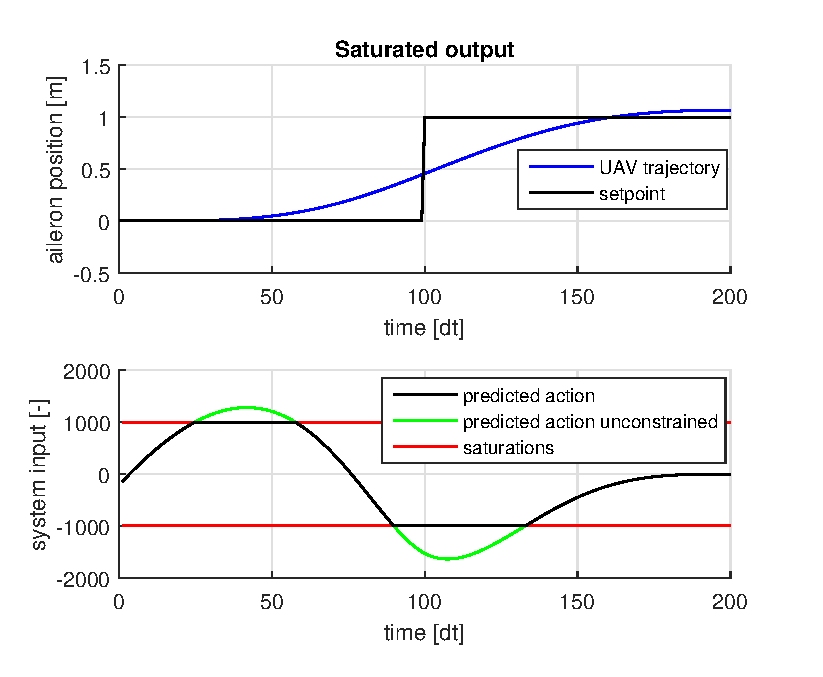
\includegraphics[width=\textwidth]{fig/step_saturated_2.eps}
	\caption{saturated MPC.}
	\label{fig:mpc_saturated}
\end{subfigure}
\caption{Step response of the system using two approaches.}
\label{fig:tricopter_px4flow}
\end{figure}

We can see in figure \ref{fig:mpc_saturated} simple saturated output. 

\section{Collision Avoidance}
\subsection{Introduction}
Collision avoidance in MPC is realized through constraining the position. This means, that we allow every predicted position to be in a certain allowed space and every violation of this space is considered to be a collision. For the UAV to get outside this allowed space will be prohibited by the algorithm used in this section. In the subsection \ref{ssec:coordinate_system} has been introduced, that the UAV is approximated with a mass point. Using this approximation would result only for the center point of the UAV not to collide. In the real world the size matters. it is not necessary to bring the whole model back. Instead the whole body can be approximated with a ring with the same center $(x, y)$ and radius $R$, such as every part of the body $(x_b, y_b)$ follows $|x - x_b, y - y_b| \leq R$. If the distance between the position of UAV and the edge of the allowed space is less or equal $R$, it can be said, that the UAV will not collide. 

The biggest problem in using MPC as a collision avoidance is creating this allowed space and converting it to the MPC constraints. 

\subsection{Convexity}
\label{sec:convexity}
Let's start with the definition of convexity. A set $S$ is convex if
\begin{equation}
\label{eq:convexity_definition}
\forall\{x_1, x_2\} \in S, \forall t \in  \textless 0, 1 \textgreater \implies t \cdot x_1 + (1-t) \cdot x_2 \in S
\end{equation}
In simple worlds, if every 2 points of a set are connected with a line, the whole line has to belong to the set.

For easily finding the global minimum of the cost function $\mathrm{J}(\underline{\textbf{u}})$, it is essential to keep the problem convex. This has many levels. First we have to ensure, that the function J is convex. This has been proven in section ???. Lets introduce a space $S$ of dimension $2T+1$, where the axes will be $(\textbf{\underline{u}}^T, z)$. Than introduce a subset $J_s$ of the space $S$ as $\{J_s \in S : \mathrm{J}(\underline{\textbf{u}}) \leq z\}$. The function $\mathrm{J}(\underline{\textbf{u}})$ is convex, if and only if the subset $J_s$ is convex. 
\subsubsection{Convexity of u}
Lets have a look at the vector $\underline{\textbf{u}}$. For MPC purposes this vector is is needed to be constrained. Because the space $S$ has one more dimension than $\underline{\textbf{u}}$, an extended version will be needed such as $(\underline{\textbf{u}}^T, z)^T$.
All points, that satisfy the condition \ref{eq:MPC_cond} will create a subset $U_s$ such as $\{U_s \in S : \textbf{A}_c \cdot \underline{\textbf{u}} \leq \textbf{B}_c\}$. The condition is independent of $z$, so it is defined for all $z$. 

We can look at this as the feasible $\underline{\textbf{u}}$ is the domain of the function $\mathrm{J}(\underline{\textbf{u}})$. Let's examine, how the $U_s$ actually looks. As mentioned in the subsection \ref{ssec:system_constraints}, the feasible $\underline{\textbf{u}}$ is an $\underline{\textbf{u}}$, that satisfies $m$ linear inequalities represented as half spaces. To satisfy all of them, set $U_s$ has to be an extended intersection of half spaces. This is important, because the convexity of set $U_s$ can be now proven. 

A theorem states, that an intersection of convex sets creates a convex set. An intersection of finite number of half spaces is a convex polytope. This polytope doesn't have to be bounded. Such a polytope is shown on a figure \ref{fig:convex_polytope} in only 2 dimensions constrained by 3 half spaces.

\begin{figure}[h]
\includegraphics[width=0.99\textwidth]{fig/convex_polytope} 
\caption{convex polytope.}
\label{fig:convex_polytope}
\end{figure}

At this time is left to prove, that a single half space is a convex set. Half space is described in equation \ref{eq:constraint_ineq_simple} as $\{\textbf{\underline{u}} : \omega_i \cdot \textbf{\underline{u}} \leq b_i$ for $i \in \{1, 2, ..., m\}\}$. If we take any 2 points $\textbf{\underline{u}}_1, \textbf{\underline{u}}_2$ belonging to the half space given by the normal vector $\omega_i$ and bias $b_i$, the line segment between them has to lie in the half space. This can be proved for any dimension. The line segment is described as

\begin{equation}
\label{eq:convex_line}
t \cdot \textbf{\underline{u}}_1 + (1-t) \cdot \textbf{\underline{u}}_2; \;\;\; t \in \textless 0, 1 \textgreater
\end{equation}

The problem of proving convexity has been transformed using the equation \ref{eq:convex_line} into equation 

\begin{equation}
\label{eq:convex_u_proof}
\omega_i \cdot (t \cdot \textbf{\underline{u}}_1 + (1-t) \cdot \textbf{\underline{u}}_2) \leq b_i
\end{equation}


An \textcolor{red}{assumption} has been made, that $\textbf{\underline{u}}_1$ and $\textbf{\underline{u}}_2$ belong to the half space, therefore 

\begin{equation}
\begin{split}
\omega_i \cdot \textbf{\underline{u}}_1 \leq b_i\\
\omega_i \cdot \textbf{\underline{u}}_2 \leq b_i.
\end{split}
\end{equation}

because $\omega_i \cdot \textbf{\underline{u}}$ is a scalar, there are just 3 possible outcomes. $\omega_i \cdot \textbf{\underline{u}}_1 = \omega_i \cdot \textbf{\underline{u}}_2$ or $\omega_i \cdot \textbf{\underline{u}}_1 < \omega_i \cdot \textbf{\underline{u}}_2$ or $\omega_i \cdot \textbf{\underline{u}}_1 > \omega_i \cdot \textbf{\underline{u}}_2$. Lets have a look at the first case $\omega_i \cdot \textbf{\underline{u}}_1 = \omega_i \cdot \textbf{\underline{u}}_2:$


\begin{equation}
\begin{split}
\omega_i \cdot (t \cdot \textbf{\underline{u}}_1 + (1-t) \cdot \textbf{\underline{u}}_2) \leq b_i\\
\omega_i \cdot (\textbf{\underline{u}}_1(t+1-t) \leq b_i\\
\omega_i \cdot \textbf{\underline{u}}_1 \leq b_i
\end{split}
\end{equation}

This case has been proven. The second case $\omega_i \cdot \textbf{\underline{u}}_1 < \omega_i \cdot \textbf{\underline{u}}_2$ is a little bit more complicated. Because $\omega_i \cdot \textbf{\underline{u}}_2 \leq b_i.$ It would be sufficient to prove 

\begin{equation}
\label{eq:conv_proof_1_less_2}
\begin{split}
\omega_i(t \cdot \textbf{\underline{u}}_1 + (1-t) \cdot \textbf{\underline{u}}_2) \leq \omega_i \cdot \textbf{\underline{u}}_2\\
\omega_i(t \cdot \textbf{\underline{u}}_1 -t \cdot \textbf{\underline{u}}_2) \leq 0\\
t \cdot \omega_i(\textbf{\underline{u}}_1 - \textbf{\underline{u}}_2) \leq 0\\
\omega_i \cdot \textbf{\underline{u}}_1 \leq \omega_i \cdot \textbf{\underline{u}}_2
\end{split}
\end{equation}

The third line has been divided by $t$. In case $t = 0$, the proof ends by $0 \leq 0$, otherwise continuing to the fourth line. This case has been also proven. Proving the last case $\omega_i \cdot \textbf{\underline{u}}_2 < \omega_i \cdot \textbf{\underline{u}}_1$ is very similar. 

\begin{equation}
\label{eq:conv_proof_2_less_1}
\begin{split}
\omega_i(t \cdot \textbf{\underline{u}}_1 + (1-t) \cdot \textbf{\underline{u}}_2) \leq \omega_i \cdot \textbf{\underline{u}}_1\\
\omega_i((t - 1) \cdot \textbf{\underline{u}}_1 - (t - 1) \cdot \textbf{\underline{u}}_2) \leq 0 \\
(t - 1) \cdot \omega_i \cdot (\textbf{\underline{u}}_1 - \textbf{\underline{u}}_2) \leq 0 \\
\omega_i \cdot \textbf{\underline{u}}_1 \leq \omega_i \cdot \textbf{\underline{u}}_2
\end{split}
\end{equation}

Similarly to the equation \ref{eq:conv_proof_1_less_2}, the third line of the equation \ref{eq:conv_proof_2_less_1} has been divided by $t-1$. 
It has been proven, that all $\textbf{\underline{u}}$, that obey the equation \ref{eq:MPC_cond} create a convex set. This means, that also the set $U_s$ is convex. Intersection of the convex set $J_s$ and $U_s$ is a convex set making the function $\mathrm{J}(\underline{\textbf{u}})$ with the domain as polytope defined $\textbf{A}_c \textbf{\underline{u}} \leq \textbf{B}_c$ is a convex function.

\section{Obstacles}
Through all this thesis, obstacles will be represented in 2D only by circles. These representations have 3 parameters: position $x_{obs}$, position $y_{obs}$ and diameter $r_{obs}$. Of course, obstacles can have various shapes, but the final allowed space will be very simplified and this is a good representation of for example people. Because the MPC runs constantly in a loop and reacts to the changing environment, it also works great with moving objects. Until now, the UAV body has been approximated with one mass point without considering the real size of the UAV. It would be difficult to calculate, whether the UAV's body has collided in the particular position or not. There is an algorithm using Minkovski Sum. Instead computing with the real size of the UAV, the representation of all obstacles will change according to the UAV's size.
Let's create a circle with the center in the UAV's center, that will completely wrap the UAV. This circle will have the smallest possible diameter $R_{UAV}$ as shown in the figure \ref{fig:UAV_dimensions}. 

\begin{figure}[h]
\begin{center}
\includegraphics[width=0.5\textwidth]{fig/UAV_dimensions} 
\caption{UAV dimensions, --template of the final picture}
\label{fig:UAV_dimensions}
\end{center}
\end{figure}

This will be a simplified representation of the UAV's body. It can be now said, that the UAV will not collide, if 

\begin{equation}
(x_{obs} - x)^2 + (y_{obs} - y)^2 \geq (R_{UAV} + r_{obs})^2.
\end{equation}

From now on we will compute with the UAV as a single mass point and every obstacle's diameter $r_{obs}$ substitute with the $r_{obs} + R_{UAV}$.	

Obstacle avoidance task is actually a task for searching a path between obstacles trying to follow a desired trajectory. From the model equation an initial condition $x_0$ and vector of input prediction $\textbf{\underline{u}}$ can be transformed as a vector of positions, velocities and accelerations at a certain predicted times. It is just positions we are interested in. 

Let's make an assumption, that the UAV's trajectory is a line created by connecting all the predicted positions. Because the UAV can not change vector of speed immediately, the real trajectory has a continuous first time derivative. Also because the second derivative is a result of the UAV's pitch and roll, which also can't be changed immediately, the second derivative is also continuous. In short, the real trajectory intersects all the predicted positions, but there is a small deviation caused by the first and second derivatives of the real system. It is very similar to approximating a function with the Taylor polynomial. To be able to approximate the real trajectory by the simplified trajectory, we need to make sure, that the predicted positions are far smaller, than the obstacles sizes. This is easy to achieve, because the time between the predicted positions is $\Delta t = 1/70s$.

Easy approach would be to say, that every trajectory is feasible, if any predicted position does not collide with any obstacle. However if the obstacle is just a simple circle in the way, the allowed space is highly non-convex. As mentioned in the section \ref{sec:convexity}, for keeping the quadratic programming convex, the allowed space for UAV has to be convex. This is the greatest disadvantage of using MPC for obstacle avoidance. 

\subsection{Creating Allowed space}

There are many ways of creating a convex space from the knowledge of the obstacles.
The approach for creating a convex allowed space is restricting any position 'behind' any obstacle. This space would be polytope defined by a set of half planes. These plains are constantly adjusting to the relative positions of the obstacles, which positions are continuously changing due to the change of the UAV position and the noise of the cameras.















-- umi se vyhybat pohybujicim se objektum
-- 2 positions in convex space -> all trajectory
-- změřit poloměr helikoptéry







\end{document}